

\tikzset{every picture/.style={line width=0.75pt}} %set default line width to 0.75pt        

\begin{tikzpicture}[x=0.75pt,y=0.75pt,yscale=-0.8,xscale=0.8]
%uncomment if require: \path (0,300); %set diagram left start at 0, and has height of 300

%Shape: Triangle [id:dp7803720964557852] 
\draw   (218.5,70) -- (353.5,208) -- (158,208) -- cycle ;
\draw  [fill={rgb, 255:red, 0; green, 0; blue, 0 }  ,fill opacity=1 ] (247,201) -- (259.5,207.5) -- (247,214) -- (253.25,207.5) -- cycle ;
\draw  [fill={rgb, 255:red, 0; green, 0; blue, 0 }  ,fill opacity=1 ] (178.47,142.57) -- (190.43,135.12) -- (189.66,149.19) -- (187.25,140.5) -- cycle ;
%Straight Lines [id:da7513488205154673] 
\draw    (158,208) -- (278.5,132) ;
\draw  [fill={rgb, 255:red, 0; green, 0; blue, 0 }  ,fill opacity=1 ] (234.46,152.5) -- (248.47,151.07) -- (241.59,163.36) -- (243.25,154.5) -- cycle ;
%Shape: Brace [id:dp6937774928119653] 
\draw   (281,130) .. controls (284.34,126.74) and (284.38,123.44) .. (281.12,120.1) -- (263.24,101.77) .. controls (258.59,97) and (257.93,92.98) .. (261.27,89.73) .. controls (257.93,92.98) and (253.93,92.23) .. (249.28,87.46)(251.37,89.6) -- (231.4,69.13) .. controls (228.14,65.79) and (224.84,65.75) .. (221.5,69) ;
%Shape: Brace [id:dp9394696690029762] 
\draw   (355,205) .. controls (358.33,201.73) and (358.37,198.43) .. (355.1,195.1) -- (331.25,170.75) .. controls (326.58,165.98) and (325.92,161.97) .. (329.25,158.71) .. controls (325.92,161.97) and (321.92,161.22) .. (317.25,156.46)(319.35,158.6) -- (293.39,132.11) .. controls (290.12,128.78) and (286.82,128.74) .. (283.49,132.01) ;
\draw  [fill={rgb, 255:red, 0; green, 0; blue, 0 }  ,fill opacity=1 ] (312.62,175.5) -- (309.06,161.86) -- (322.26,166.78) -- (313.25,166.5) -- cycle ;
%Straight Lines [id:da7583773908360483] 
\draw    (431,82) -- (457.02,105.65) ;
\draw [shift={(458.5,107)}, rotate = 222.27] [color={rgb, 255:red, 0; green, 0; blue, 0 }  ][line width=0.75]    (10.93,-3.29) .. controls (6.95,-1.4) and (3.31,-0.3) .. (0,0) .. controls (3.31,0.3) and (6.95,1.4) .. (10.93,3.29)   ;
%Straight Lines [id:da19534068791687043] 
\draw    (430.5,105.5) -- (457.42,84.72) ;
\draw [shift={(459,83.5)}, rotate = 502.33] [color={rgb, 255:red, 0; green, 0; blue, 0 }  ][line width=0.75]    (10.93,-3.29) .. controls (6.95,-1.4) and (3.31,-0.3) .. (0,0) .. controls (3.31,0.3) and (6.95,1.4) .. (10.93,3.29)   ;

% Text Node
\draw (138,204.4) node [anchor=north west][inner sep=0.75pt]    {$O$};
% Text Node
\draw (360,202.4) node [anchor=north west][inner sep=0.75pt]    {$A$};
% Text Node
\draw (214,48.4) node [anchor=north west][inner sep=0.75pt]    {$B$};
% Text Node
\draw (261,210.4) node [anchor=north west][inner sep=0.75pt]    {$\underline{a}$};
% Text Node
\draw (164,109.4) node [anchor=north west][inner sep=0.75pt]    {$\underline{b}$};
% Text Node
\draw (218,140.4) node [anchor=north west][inner sep=0.75pt]    {$\underline{c}$};
% Text Node
\draw (286,112.4) node [anchor=north west][inner sep=0.75pt]    {$C$};
% Text Node
\draw (263,72.4) node [anchor=north west][inner sep=0.75pt]    {$n$};
% Text Node
\draw (332,144.4) node [anchor=north west][inner sep=0.75pt]    {$m$};
% Text Node
\draw (388,141.4) node [anchor=north west][inner sep=0.75pt]    {$\underline{c} =\dfrac{m\underline{b} +n\underline{a}}{m+n}$};
% Text Node
\draw (413,65.4) node [anchor=north west][inner sep=0.75pt]    {$m$};
% Text Node
\draw (460,65.4) node [anchor=north west][inner sep=0.75pt]    {$n$};
% Text Node
\draw (415,100.4) node [anchor=north west][inner sep=0.75pt]    {$\underline{a}$};
% Text Node
\draw (460,102.4) node [anchor=north west][inner sep=0.75pt]    {$\underline{b}$};


\end{tikzpicture}